\chapter{Konzept}

Das Kapitel Konzeption beschäftigt sich zunächst mit dem Prozess der Feature Extraktion. Hierfür wird der SIFT Algorithmus nach Lowe genutzt. Darauf aufbauend werden zwei Verfahren vorgestellt, das Bag of Visual Words Modell und der Autoencoder, die anhand von SIFT Deskriptoren eine Klassifizierung von Bildern ermöglichen.

\begin{enumerate}
	\item Verarbeitung der bestehenden Bilder
	\item Auswahl der Features
	\item Layer des Netzes, Stacking, Denoising ?	
\end{enumerate}

\section{Feature Extraktion}

Die Extraktion der Features ist die Basis für beide Varianten der Klassifizierung. Das Bag of Visual Words Modell nutzt die von SIFT erzeugten Feature Deskriptor für die weitere Verarbeitung. Der Autoencoder hingegen arbeitet mit Gradienten der \textit{keypoints} die vom SIFT Detektor ermittelt wurden. Aus diesem Grund werden die Feature-Vektoren und \textit{keypoints} beide berechnet und getrennt gespeichert.
Der SIFT Deskriptor enthält 128 Dimensionen und ist so für einen Vergleich nur schwer geeignet, da pro Bild ca. 100 bis 1000 Feature Vektoren generiert werden. Es werden daher im folgenden zwei Ansätze vorgestellt, die die Dimensionalität der Features reduzieren und eine durch Grafikkarten gestützte Berechnung von ähnlichen Bildern ermöglichen.

\begin{enumerate}
	\item Hier nochmal etwas auf SIFT eingehen (Funktionsweise)?
	\item Mehr zum Prozess sagen? Woher die Bilder kommen
	\item TODO: Wie werden Bilder gespeichert? Format, Platte / DB?
\end{enumerate}

\section{Ansatz 1: Bag of Visual Words}

Der erste Ansatz verfolgt das Visual Words Modell. Im ersten Schritt muss ein Codebook generiert werden, dass als Modell dient um die Bilder zu klassifizieren. Hierfür werden die Feature-Vektoren der Trainingsbilder zunächst durch einen k-means Algorithmus quantisiert.

Sobald das Codebook erzeugt wurde, kann durch einen Histogramm Algorithmus die Berechnung erfolgen. In der Analyse wurde betrachtet, welcher Teile des Bag of Visual Word Modells sich parallelisieren lassen. wie sich ein Histogramm parallel auf Nvidia Grafikkarten berechnen lässt. 

\begin{enumerate}
	\item hier könnte ich gut auf den Aufbau eingehen (CPU ist master, bereitet Daten vor, cuda führt Distanzberechnung / Reduktion aus.), oder ist cuda eher Implementierungssache?
	\item hier vorhandene Implementierungen von k-means erwähnen?
	\item Wie wird klassifiziert?
\end{enumerate}

\section{Aufbau des Autoencoders}

In diesem Ansatz werden zur Reduzierung der Dimensionen der Feature-Vektoren wird ein Stacked Denoising Autoencoder verwendet wie er in der Arbeit von TODO \cite{aed2016} vorgeschlagen wurde. Der Autoencoder soll eine komprimierte Darstellung der Gradientenvektoren erzielen, die aus den \textit{intereset points} berechnet werden. Da dieser Vektor 3042 Werte enthält, besitzt der Autoencoder in der Eingabeschicht 3042 Neuronen. Der Encoder des vorgeschlagenen Modells besteht aus fünf Schichten, deren Neuronenanzahl sukzessive reduziert wird, bis schließlich eine Darstellung in 36 Dimensionen erreicht wird. Abbildung \ref{img:ae_model} zeigt die Schichten des Autoencoders.

\begin{figure}
	\centering
	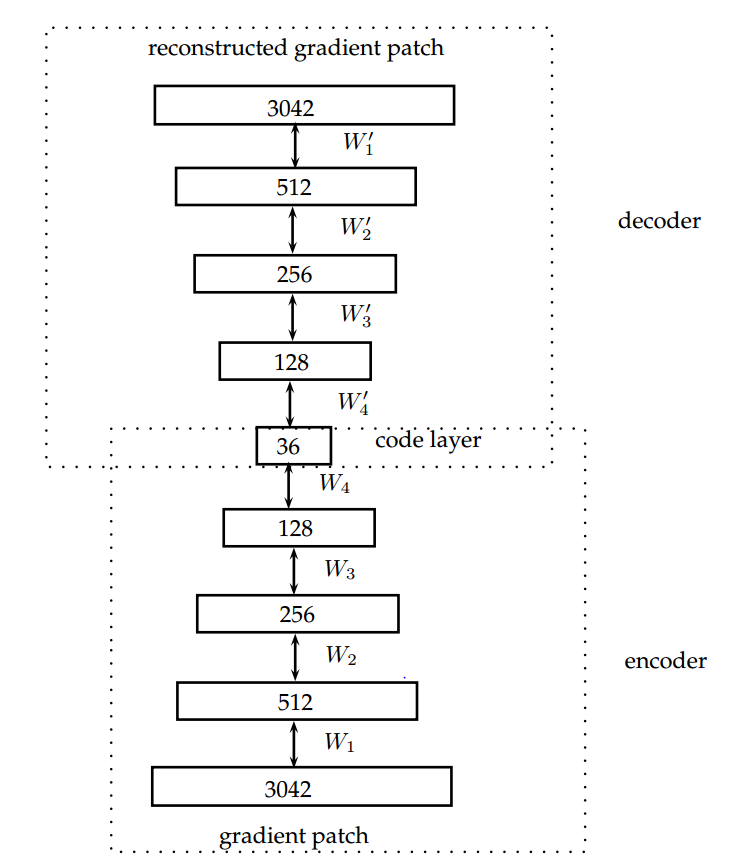
\includegraphics[scale=0.6]{images/ae_model.png}
	\caption{Schichten des verwendeten Autoencoders, Abbildung aus \cite{aed2016}}
	\label{img:ae_model}
\end{figure}

\begin{itemize}
	\item Mit Referenz auf die Arbeit ist es plausibel dieses Modell zu verwenden?
	\item In der Konzeption bereits TensorFlow erwähnen und somit Beschleunigung durch cuda Bindings?
\end{itemize}